\chapter{Event selection}
The event selection has been optimized in order to maximize the signal significance of the signal over backgraound.
The whole event selection of the analysis is shown in this chapter.

First the preselection cuts are applied including basic event cleaning and the trigger requirements, then the specific event selection is applied to the each 0,1,2-lepton channels.
For the main event selection, first the selection of the one $W/Z$ boson decaying leptonically is selected. Then in each channel, the forward jets and the hadronically decaying boson is selected, and the selection to enhance the VBS topology is applied.

%\section{Object selection}
%The selection of the physics objects (electron, muon, jet, and missing transverse energy) is described in this section.
%\subsection{Electrons and Muons}
%The used electron working point described in Section\ref{} is shown.
%\begin{itemize}
%    \item "Tight" electron (muon) for selecting $W \rightarrow e\nu$ candidate in 1-lepton channel
%    \item "Loose" electron (muon) for selecting $Z \rightarrow e^\plus e^\minum$ candidate in 2-lepton channel \\ 
%   for vetoing events with additional leptons in 0-lepton and 1-lepton channel.
%\end{itemize}
%In 2-lepton channel, "Loose" electron (muon) is used which means looser isolation working point is used to keep high signal efficiency at high-$p_T$ region since there are two electron candidates to be close each other.
%The common jet selection criteria for small-R jets, are $>20 \mathrm{GeV}(|\eta|<2.5)$ and $>30 \mathrm{GeV}(2.5<|\eta|<4.5)$. For Large-R jets, 

\section{0-lepton}
The $Z \rightarrow \nu\nu$ identification requires no Loose lepton and high missing energy (E$_T^{miss}$ > 200~GeV) in the final state. There are significant QCD multijet background in 0-lepton channel, therefore some cuts suppressing the multijets are applied: \\
\\
- $p_{\mathrm{T}}^{\mathrm{miss}}>50 \mathrm{GeV}$ \\
- $\Delta \phi\left(E_{\mathrm{T}}^{\mathrm{miss}}, p_{\mathrm{T}}^{\mathrm{miss}}\right)<\pi / 2$ \\
- $\min \left(\Delta \phi\left(E_{\mathrm{T}}^{\mathrm{miss}}, j\right)\right)>\pi / 6$ \\
- $\Delta \phi\left(E_{\mathrm{T}}^{\mathrm{miss}}, \overrightarrow{\mathbf{V}}_{\mathrm{had}}\right)>\pi / 9$ \\
where $p_{\mathrm{T}}^{\mathrm{miss}}$ is the track-based missing momentum, and $\min \left(\Delta \phi\left(E_{\mathrm{T}}^{\mathrm{miss}}, j\right)\right)$ is the minimum azimuthal difference betwween $E_{\mathrm{T}}^{\mathrm{miss}}$ and small-R jets.

\section{1-lepton}
To select the events with $W \rightarrow l\nu$ candidate, exactly one Tight lepton is required.
In order to suppress the multi-jet background, following cuts are applied for all regions: \\
- $E_{\mathrm{T}}^{\text {miss }}>80 \mathrm{GeV}$ \\ \\
- $p_{\mathrm{T}, \ell}>28 \mathrm{GeV}$ \\
- $m_{J}>50 \mathrm{GeV}$ (merged only) \\

\section{2-lepton}
The $Z \rightarrow ll$ candidates are selected by requiring two isolated same-flavour Loose leptons. Both leptons required to be $p_T$ > 27~GeV. Opposite charges are required only for muons and not for electrons, since electrons are more sensitive to charge mis-identification due to the conversions of photons from bremsstrahlung, especially at high $E_T$.
The $m_{ll}$, invariant mass of the dilepton is required to be in the mass window \\ \\
- $83 < m_{ee}< 99~GeV$ \\ 
- $\left(85.6-0.0117 p_{\mathrm{T}, \ell \ell}\right)<m_{\mu \mu}<\left(94.0+0.0185 p_{\mathrm{T}, \ell \ell}\right) \mathrm{GeV}$ \\
The second equation for muons was oprimized from the 2015$\plus$16 analysis~\cite{}. 
The modeling distribution of lepton distribution in the early stage of the selection is shown in Figure~\ref{fig:2lepLeptons}. The mass peak of Z boson can be seen here.

\begin{figure}[ht]
    \centering
    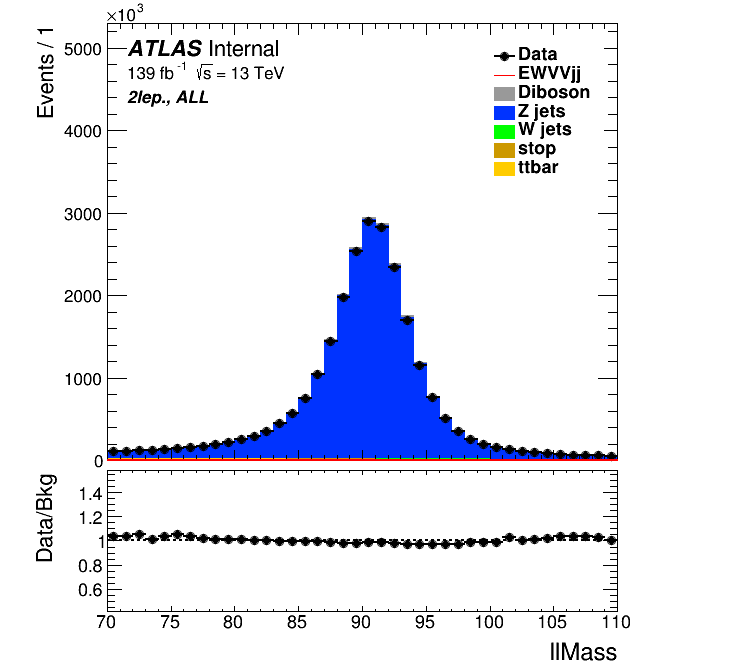
\includegraphics[width=0.3\textwidth]{figures/2lep/dataMC/C_0ptag1pfat0pjet_0ptv_ALL_llMass_Lin.png}
    \caption{Lepton distributions in 2-lepton channel. The events before any selections are shown. Z mass peak is shown in $M_{ll}$ distribution.}
    \label{fig:2lepLeptons}
\end{figure}


\begin{table}[h]
  \caption{List of the \textbf{pre-selections applied in the CxAOD framework} to reduce the data size.
Definitions of Tight and Loose leptons are found in Sections~\ref{subsec:electron_selection}--\ref{subsec:muon_selection}.
$N_j$ is the number of signal- and VBF-jets defined in Section~\ref{subsec:jet_selection}.
$N_J^{\textrm{LCTopo}}$ is the number of large-R jets with $\pt>200\,\GeV$ and $\left| \eta \right| < 2.5$.
} \label{tab:presel_CxAOD}

\begin{center}
\resizebox{0.7\textwidth}{!}{
\begin{tabular}{|l|c|}
\hline\hline
\multicolumn{2}{|c|}{ Common } \\
\hline\hline
Trigger & listed in Table~\ref{tab:triggers} \\
\hline
Event Cleaning & listed in Section~\ref{subsec:event_cleaning} \\
\hline
Number of jets & $N_j \geq 2$ or $N_J^{\textrm{LCTopo}} \geq 1$ \\
\hline\hline\hline
\multicolumn{2}{|c|}{ 1-lepton channel } \\
\hline
Number of Tight leptons   & $=1$ \\
\hline
Number of additional Loose leptons   & $=0$ \\
\hline
\ptlv                     & $>75\,\GeV$ \\
\hline\hline
\multicolumn{2}{|c|}{ 2-lepton channel } \\
\hline\hline
Number of Loose leptons   & $=2$ \\
\hline
The leading lepton \pt    & $> 25\,\GeV$ \\
\hline\hline
\multicolumn{2}{|c|}{ 0-lepton channel } \\
\hline\hline
Number of Loose leptons   & $= 0$ \\
\hline
\met                      & $> 140\,\GeV$ \\
\hline\hline
\end{tabular}
}
\end{center}
\end{table}



%Event selection
\section{Event Selection}

The selections applied are summarized here in tables
\ref{tab:0lep_merged}-\ref{tab:0lep_resolved}
\ref{tab:1lep_merged}-\ref{tab:1lep_resolved}
\ref{tab:2lep_merged}-\ref{tab:2lep_resolved}

%%% 0-lepton channel
\begin{table}[ht!]
\small
\caption{A summary of regions event selection for \zlep channel in the merged regime.}
\label{tab:0lep_merged}
\begin{center}
\resizebox{\textwidth}{!}{
\begin{tabular}{|l|l|c|c|c|}
\hline
\multicolumn{2}{|l|}{\multirow{2}{*}{Selection}} & \multicolumn{2}{c|}{SR}  &  $V$ CR \\
\cline{3-5}
\multicolumn{2}{|l|}{} & HP & LP & inclusive \\
\hline
\multirow{3}{*}{$Z \to \nu\nu$}  &  Number of Loose leptons & \multicolumn{3}{c|}{0} \\
\cline{2-5}
    & \met                                     & \multicolumn{3}{c|}{ > 200 GeV }                  \\
\cline{2-5}
    & \mpt                                     & \multicolumn{3}{c|}{ > 50 GeV}                    \\
\hline

\multirow{3}{*}{anti-QCD}  & min($\Delta\Phi$(\met,small-R jets))     & \multicolumn{3}{c|}{ $> \pi/6$} \\
\cline{2-5}
    & $\Delta\Phi$(\met,\mpt)                  & \multicolumn{3}{c|}{ $< \pi/2$}                   \\
\cline{2-5}
    & $\Delta\phi(\met, Sig-J)$                & \multicolumn{3}{c|}{ $> \pi/9$}                   \\
\hline
\multirow{3}{*}{VBS jets candidates} & Leading Tag jet \pt & \multicolumn{3}{c|}{ $>30\,\GeV$ } \\
\cline{2-5}
                          & Subleading Tag jet \pt & \multicolumn{3}{c|}{ $>30\,\GeV$ }\\
\cline{2-5}
                          & $m_{jj}$ & \multicolumn{3}{c|}{ $> 400 \GeV$ } \\
\hline
\multirow{2}{*}{$W/Z \to J$} & Num of large-R jets & \multicolumn{3}{c|}{$\geq 1$} \\
\cline{2-5}
& 3-Var Tagger & pass50WP & pass80WP \&\& !pass50WP & fail80WP \\
\hline
\end{tabular}
}
\end{center}
\end{table}


\begin{table}[ht!]
\small
\caption{A summary of regions event selection for \zlep channel in the resolved regime.}
\label{tab:0lep_resolved}
\begin{center}
\resizebox{\textwidth}{!}{
\begin{tabular}{|l|l|c|c|}
\hline
\multicolumn{2}{|l|}{Selection} & SR  & $V$ CR \\
\hline
\multirow{3}{*}{$Z \to \nu\nu$}  &  Number of Loose leptons & \multicolumn{2}{c|}{0} \\
\cline{2-4}
    & \met                                     & \multicolumn{2}{c|}{ > 200 GeV }                  \\
\cline{2-4}
    & \mpt                                     & \multicolumn{2}{c|}{ > 50 GeV}                    \\
\hline

\multirow{3}{*}{anti-QCD}  & min($\Delta\Phi$(\met,small-R jets))     & \multicolumn{2}{c|}{ $> \pi/6$} \\
\cline{2-4}
    & $\Delta\Phi$(\met,\mpt)                  & \multicolumn{2}{c|}{ $< \pi/2$}                   \\
\cline{2-4}
    & $\Delta\phi(\met, Sig-J)$                & \multicolumn{2}{c|}{ $> \pi/9$}                   \\
\hline
\multirow{3}{*}{VBS jets candidates} & Leading Tag jet \pt & \multicolumn{2}{c|}{ $>30\,\GeV$ } \\
\cline{2-4}
                          & Subleading Tag jet \pt & \multicolumn{2}{c|}{ $>30\,\GeV$ }\\
\cline{2-4}
                          & $m_{jj}$ & \multicolumn{2}{c|}{ $> 400 \GeV$ } \\
\hline
\multirow{4}{*}{$W/Z \to jj$} & Num of signal small-R jets & \multicolumn{2}{c|}{2} \\
\cline{2-4}
              & Leading signal jet \pt & \multicolumn{2}{c|}{ $>40\,\GeV$ }\\
\cline{2-4}
              & Subleading signal jet \pt & \multicolumn{2}{c|}{ $>20\,\GeV$ }\\
\cline{2-4}
              &$Z \to q\bar{q}$ and $W \to q\bar{q}$     &   $64 < m_{jj} < 106 \gev$ & $50<m_{jj}<64 \,GeV$ or $m_{jj}>106$ \\
\hline
VBS enhancing & $m_{jjj}$ & \multicolumn{2}{c|}{ $>220$~GeV} \\
\hline
\end{tabular}
}
\end{center}
\end{table}

%%% 1-lepton channel
\begin{table}[t]
  \caption{A summary of regions event selection for \olep channel in the resolved regime.}
\label{tab:1lep_resolved}
\begin{center}
\resizebox{\textwidth}{!}{
\begin{tabular}{|l|l|c|c|c|}
\hline
\multicolumn{2}{|l|}{cuts} & SR & $W$ CR (WR) & \ttbar CR (TR) \\
\hline
\multirow{4}{*}{$W\rightarrow \ell\nu$ } & Number of Tight leptons & \multicolumn{3}{c|}{ 1 } \\
\cline{2-5}
&Number of Loose leptons & \multicolumn{3}{c|}{ 0 }  \\
\cline{2-5}
&\met & \multicolumn{3}{c|}{ $>80\,\GeV$ } \\
\cline{2-5}
&$\pt(\ell)$ & \multicolumn{3}{c|}{ $>30\,\GeV$ } \\
\hline
\multirow{3}{*}{VBS jets candidates} & Leading Tag jet \pt & \multicolumn{3}{c|}{ $>30\,\GeV$ } \\
\cline{2-5}
                          & Subleading Tag jet \pt & \multicolumn{3}{c|}{ $>30\,\GeV$ }\\
\cline{2-5}
                          & $m_{jj}$ & \multicolumn{3}{c|}{ $> 400 \GeV$ } \\
\hline
\multirow{4}{*}{$W/Z\rightarrow jj$ } & Number of small-R jets & \multicolumn{3}{c|}{ $\geq 4$ } \\ %$\geq 2$ & $\geq 2$ & $\geq 2$  \\
\cline{2-5}
& Leading jet \pt & \multicolumn{3}{c|}{ $>40$~GeV}\\
\cline{2-5}
& Subleading jet \pt & \multicolumn{3}{c|}{ $>20$~GeV}\\
\cline{2-5}
 &$Z \to q\bar{q}$ and $W \to q\bar{q}$     &   $64 < m_{jj} < 106 \gev$ & $50<m_{jj}<64 \,GeV$ or $m_{jj}>106$ & $64 < m_{jj} < 106 \gev$ \\
\hline
Top veto &  Number of additional $b$-tagged jets & \multicolumn{2}{c|}{0} & $\geq 1$ \\
\hline
VBS enhancing & $m_{jjj}$ & \multicolumn{3}{c|}{ $>220$~GeV} \\
\hline
\end{tabular}
}
\end{center}
\end{table}

\begin{table}[t]
\caption{A summary of regions event selection for \olep channel in the merged regime.}
\label{tab:1lep_merged}
\begin{center}
\resizebox{\textwidth}{!}{
\begin{tabular}{|l|l|c|c|c|c|c|}
\hline
\multicolumn{2}{|l|}{\multirow{2}{*}{Selection}} & \multicolumn{2}{c|}{SR}  &  $W$ CR (WR)  & \multicolumn{2}{c|}{$t\bar{t}$ CR (TR)} \\
\cline{3-7}
\multicolumn{2}{|l|}{} & HP & LP & incl & HP & LP \\
\hline
\multirow{4}{*}{$W\rightarrow \ell\nu$} & Num of Tight leptons & \multicolumn{5}{c|}{ 1 } \\
\cline{2-7}
&Num of Loose leptons & \multicolumn{5}{c|}{ 0 }  \\
\cline{2-7}
&\vphantom{\Large B} \met & \multicolumn{5}{c|}{ $>80\,\GeV$ } \\
\cline{2-7}
&$\pt(\ell)$ & \multicolumn{5}{c|}{ $>30\,\GeV$ } \\
\hline
\multirow{3}{*}{VBS jets candidates} & Leading Tag jet \pt & \multicolumn{5}{c|}{ $>30\,\GeV$ } \\
\cline{2-7}
                          & Subleading Tag jet \pt & \multicolumn{5}{c|}{ $>30\,\GeV$ }\\
\cline{2-7}
                          & $m_{jj}$ & \multicolumn{5}{c|}{ $> 400 \GeV$ } \\
\hline
\multirow{2}{*}{$W/Z\rightarrow J$} & Num of large-$R$ jets & \multicolumn{5}{c|}{ $\geq 1$ } \\
\cline{2-7}
& 3-Var Tagger & pass50WP & pass80WP \&\& !pass50WP & fail80WP & pass50WP & pass80WP \&\& !pass50WP \\
%& \vphantom{\Large B} $D_2/n_{Tracks}$ cut & pass & fail & pass & fail & pass & fail \\
%\cline{2-8}
%& $W/Z$ mass window cut & pass & pass & fail & fail & pass & pass\\
\hline
Top veto & Num of $b$-tagged jets outside of large-R jet & \multicolumn{3}{c|}{0} & \multicolumn{2}{c|}{$\geq 1$} \\
\hline
\end{tabular}
}
\end{center}
\end{table}

%%% 2-leptons channel
\begin{table}[ht!]
\small
\caption{A summary of regions event selection for 2-lepton channel in the merged regime.}
\label{tab:2lep_merged}
\begin{center}
\resizebox{\textwidth}{!}{
\begin{tabular}{|l|l|c|c|c|}
\hline
\multicolumn{2}{|l|}{\multirow{2}{*}{Selection}} & \multicolumn{2}{c|}{SR}  &  $Z$ CR \\
\cline{3-5}
\multicolumn{2}{|l|}{} & HP & LP & incl \\
\hline
\multirow{6}{*}{$Z \to \ell\ell$}  &  Number of Loose leptons & \multicolumn{3}{c|}{2} \\
\cline{2-5}
                          & Same flavor &  \multicolumn{3}{c|}{yes} \\
\cline{2-5}
                          & Leading lepton \pt  & \multicolumn{3}{c|}{$>27\,\GeV$} \\
\cline{2-5}
                          & Subleading lepton \pt  & \multicolumn{3}{c|}{$>27\,\GeV$} \\
\cline{2-5}
                          & \multirow{2}{*}{dilepton invariant mass} & \multicolumn{3}{c|}{$ 83 < m_{ee} < 99 \gev$} \\
                          &  & \multicolumn{3}{c|}{$-0.01170\ptll+85.63 < m_{\mu\mu} < 0.01850\ptll+94.00 \gev$} \\
\cline{2-5}
                          & Opposite sign &  \multicolumn{3}{c|}{For $\mu\mu$ channel only} \\
\hline
\multirow{3}{*}{VBS jets candidates} & Leading Tag jet \pt & \multicolumn{3}{c|}{ $>30\,\GeV$ } \\
\cline{2-5}
                          & Subleading Tag jet \pt & \multicolumn{3}{c|}{ $>30\,\GeV$ }\\
\cline{2-5}
                          & $m_{jj}$ & \multicolumn{3}{c|}{ $> 400 \GeV$ } \\
\hline
\multirow{2}{*}{$W/Z \to J$} & Num of large-R jets & \multicolumn{3}{c|}{$\geq 1$} \\
\cline{2-5}
& 3-Var Tagger & pass50WP & pass80WP \&\& !pass50WP & fail80WP \\
\hline
\end{tabular}
}
\end{center}
\end{table}

\begin{table}[ht!]
\small
\caption{A summary of regions event selection for \tlep channel in the resolved regime.}
\label{tab:2lep_resolved}
\begin{center}
\resizebox{\textwidth}{!}{
\begin{tabular}{|l|l|c|c|}
\hline
\multicolumn{2}{|l|}{Selection} & SR  & $Z$ CR \\
\hline
\multirow{6}{*}{$Z \to \ell\ell$}  &  Number of Loose leptons & \multicolumn{2}{c|}{2} \\
\cline{2-4}
                          & Same flavor &  \multicolumn{2}{c|}{yes} \\
\cline{2-4}
                          & Leading lepton \pt  & \multicolumn{2}{c|}{$>27\,\GeV$} \\
\cline{2-4}
                          & Subleading lepton \pt  & \multicolumn{2}{c|}{$>27\,\GeV$} \\
\cline{2-4}
                          & \multirow{2}{*}{dilepton invariant mass} & \multicolumn{2}{c|}{$ 83 < m_{ee} < 99 \gev$} \\
                          & & \multicolumn{2}{c|}{$-0.01170\ptll+85.63 < m_{\mu\mu} < 0.01850\ptll+94.00 \gev$} \\
\cline{2-4}
                          & Opposite sign &  \multicolumn{2}{c|}{For $\mu\mu$ channel only} \\
\hline
\multirow{3}{*}{VBS jets candidates} & Leading Tag jet \pt & \multicolumn{2}{c|}{ $>30\,\GeV$ } \\\cline{2-4}
                          & Subleading Tag jet \pt & \multicolumn{2}{c|}{ $>30\,\GeV$ }\\
\cline{2-4}
                          & $m_{jj}$ & \multicolumn{2}{c|}{ $> 400 \GeV$ } \\
\hline
\multirow{4}{*}{$W/Z \to jj$} & Num of signal small-R jets & \multicolumn{2}{c|}{2} \\
\cline{2-4}
              & Leading signal jet \pt & \multicolumn{2}{c|}{ $>40\,\GeV$ }\\
\cline{2-4}
              & Subleading signal jet \pt & \multicolumn{2}{c|}{ $>20\,\GeV$ }\\
\cline{2-4}
              &$Z \to q\bar{q}$ and $W \to q\bar{q}$     &   $64 < m_{jj} < 106 \gev$ & $50<m_{jj}<64 \,GeV$ or $m_{jj}>106$ \\
\hline
VBS enhancing & $m_{jjj}$ & \multicolumn{2}{c|}{ $>220$~GeV} \\
\hline
\end{tabular}
}
\end{center}
\end{table}
